\documentclass{article}

\usepackage[utf8]{inputenc}
\usepackage{t1enc}
\usepackage[magyar]{babel}
\sloppy

\usepackage{tikz}

\author{Endrey Márk}
\title{Ész Ventura\\98.~feladvány: Bombonyok\\\large Játssz bombonnyal, és nyerj csokit!}

\newcommand{\anz}[1]{$\mathrm{I}_{#1}$}
\newcommand{\nch}[1]{$\mathrm{II}_{#1}$}

\begin{document}
	\maketitle
	\tableofcontents
	\section{Elvek és építőelemek}
		Adjunk általánosabb nevet Boginak és Máténak! Bogi a Kezdőjátékos (,,die Anziehende''), Máté pedig a ,,Követő'' (utánalépő) játékos (,,der Nachziehende'').
		Ezek a nevek (különösen a német megfogalmazás) sokat fognak segíteni majd a szimmetriaelvek felismerésében, megfogalmazásában.
		A játék természetétéből fakadóan nincs döntetlen stratégia, így vagy Kezdő, vagy Követő játékosnak van nyerési stratégiája.
		\subsection{Kisméretű példák}
			\subsubsection{A $2\times2$ eset mint később fontos általánosítási lehetőség}
				A ,,sortöltés'' mint kezdőlépés vereséghez vezet (márming ha Követő ezt kihsználja):\\
				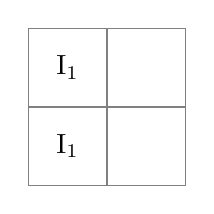
\begin{tikzpicture}
					\draw[step=1cm, color=gray] (-1, -1) grid (1, 1);
					\node at (-0.5, -0.5) {\anz1};
					\node at (-0.5,  0.5) {\anz1};
				\end{tikzpicture}
				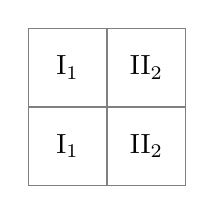
\begin{tikzpicture}
					\draw[step=1cm, color=gray] (-1, -1) grid (1, 1);
					\node at (-0.5, -0.5) {\anz1};
					\node at (-0.5,  0.5) {\anz1};
					\node at ( 0.5, -0.5) {\nch2};
					\node at ( 0.5,  0.5) {\nch2};
				\end{tikzpicture}
				
				A lényegesen különböző egyetlen alternatíva a ,,sarokkezdés'', ez viszont Követőt a ,,pepita'' válaszlépésre fogja kényszeríteni, mert ha Követő nem-pepitán reagálna, veszítene:\\
				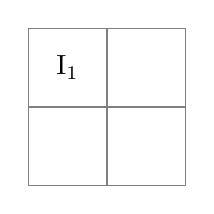
\begin{tikzpicture}
					\draw[step=1cm, color=gray] (-1, -1) grid (1, 1);
					\node at (-0.5,  0.5) {\anz1};
				\end{tikzpicture}
				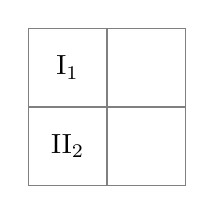
\begin{tikzpicture}
					\draw[step=1cm, color=gray] (-1, -1) grid (1, 1);
					\node at (-0.5,  0.5) {\anz1};
					\node at (-0.5, -0.5) {\nch2};
				\end{tikzpicture}
				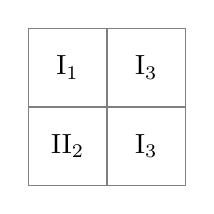
\begin{tikzpicture}
					\draw[step=1cm, color=gray] (-1, -1) grid (1, 1);
					\node at (-0.5,  0.5) {\anz1};
					\node at (-0.5, -0.5) {\nch2};
					\node at ( 0.5, -0.5) {\anz3};
					\node at ( 0.5,  0.5) {\anz3};
				\end{tikzpicture}

				Követőjátékos tehát  Kezdőjátékos ,,sarokkezdésére'' a ,,pepita'' válaszlépést fogja adni, innen pedig neki (Követőnek) nyerő sratégiája van:\\
				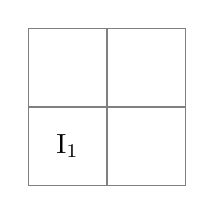
\begin{tikzpicture}
					\draw[step=1cm, color=gray] (-1, -1) grid (1, 1);
					\node at (-0.5, -0.5) {\anz1};
				\end{tikzpicture}
				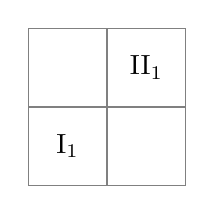
\begin{tikzpicture}
					\draw[step=1cm, color=gray] (-1, -1) grid (1, 1);
					\node at (-0.5, -0.5) {\anz1};
					\node at ( 0.5,  0.5) {\nch1};
				\end{tikzpicture}
				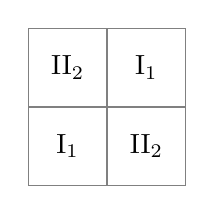
\begin{tikzpicture}
					\draw[step=1cm, color=gray] (-1, -1) grid (1, 1);
					\node at (-0.5, -0.5) {\anz1};
					\node at ( 0.5,  0.5) {\anz1};
					\node at ( 0.5, -0.5) {\nch2};
					\node at (-0.5,  0.5) {\nch2};
				\end{tikzpicture}

				Kezdőjátékosnak tehát sem a ,,sorkitöltős'', sem a ,,sarokkezdős'' kezsőlépéssel nincs nyerő stratégiája, más (lényegesen különböző, nem-ekvivalens) kezdőlépés pedig nem létezik ilyen kicsiny ($2\times2$-es) táblán. A $2\times2$-es játék tehát Követő számára nyújt nyerő stratégiát.
		\subsection{Visszalépés elv, relativitás}
		\subsection{Abszolút elvek}
			\subsubsection{A tengelyes tükrözés, fizikai tengely}
			\subsubsection{A középpontos tükrözés, nem-fizikai középpont}
	\section{Összefoglalás}
		\subsection{Esetek}
		\subsection{Levezetési nyelvtan}
\end{document}
